%Master File:lectures.tex

\lesson{Boosting}
\vspace{-1cm}
\begin{center}
  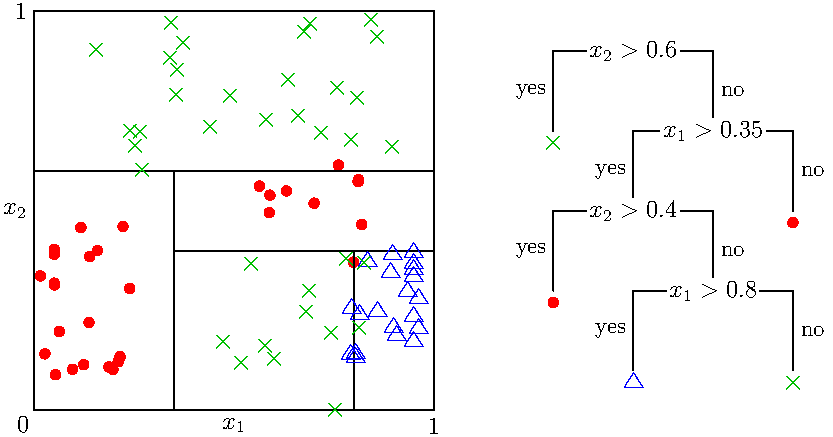
\includegraphics[height=12cm]{decisionTree-5}
\end{center}

\keywords{Boosting, AdaBoost, Gradient Boosting}


%%%%%%%%%%%%%%%%%%%%%%% Next Slide %%%%%%%%%%%%%%%%%%%%%%%
\renewcommand{\Outline}{%
\begin{slide}
\section[1]{Outline}

\begin{minipage}{8cm}\raggedright
  \begin{enumerate}
    \outlineitem{Boosting}{boosting}
    \outlineitem{AdaBoost}{adaboost}
    \outlineitem{Gradient Boosting}{gradientboosting}
  \end{enumerate}
\end{minipage}\hfill
\begin{minipage}{15cm}
  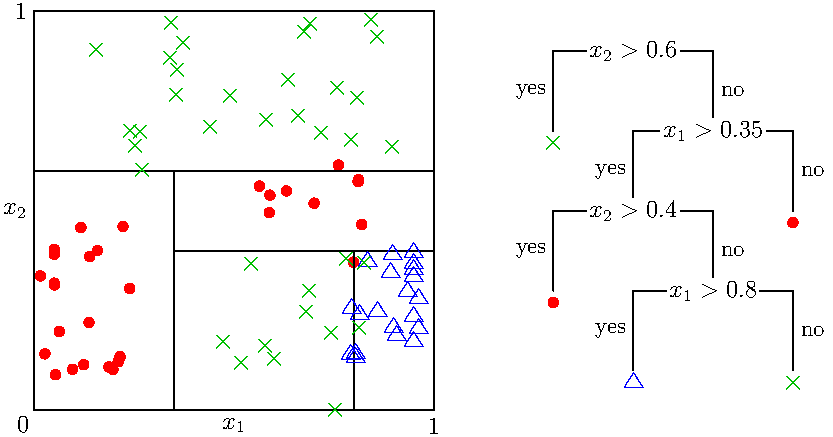
\includegraphics[width=15cm]{decisionTree-5}
\end{minipage}
\end{slide}
\addtocounter{outlineitem}{1}
}

\setcounter{outlineitem}{1}

%%%%%%%%%%%%%%%%%%%%%%% Next Slide %%%%%%%%%%%%%%%%%%%%%%%
\Outline %   Boosting
\toptarget{firstoutline}
%%%%%%%%%%%%%%%%%%%%%%% Next Slide %%%%%%%%%%%%%%%%%%%%%%%

\begin{slide}
\section{Boosting}

\begin{PauseHighLight}
  \begin{itemize}
  \item In boosting we make a \emph{strong learner} by using a weighted
    sum of \emph{weak learners}
    \begin{align*}
      C_n(\bm{x}) = \sum_{i=1}^n \alpha_i \, \hat{h}_i(\bm{x})\pause
    \end{align*}
  \item Weak learners, $\hat{h}_i(\bm{x})$, are learning machine that do a
    little better than chance\pause
  \item The trick is to choose the weights, $\alpha_i$\pause
  \item Because the weak learners do little better than chance we
    (miraculously) \textbf{don't} overfit\pause{} that much\pauseb
  \end{itemize}
\end{PauseHighLight}

\end{slide}

%%%%%%%%%%%%%%%%%%%%%%% Next Slide %%%%%%%%%%%%%%%%%%%%%%%

\begin{slide}
\section{Shallow Trees}

\begin{PauseHighLight}
  \begin{itemize}
  \item One of the most effective type of weak learner are very shallow
    trees\pause
  \item Sometimes we just use one variable (the stump)\pause, although
    usually we would use slightly deeper trees\pauseb
  \item There are different algorithms for choosing the weights
    \begin{itemize}
    \item adaboost\pause---a classic algorithm for binary classification\pauseb
    \item gradient boosting\pause---used for regression, trains a
      weak learner on the residual errors\pauseb
    \end{itemize}
  \end{itemize}
\end{PauseHighLight}

\end{slide}
%%%%%%%%%%%%%%%%%%%%%%% Next Slide %%%%%%%%%%%%%%%%%%%%%%%
\Outline %   Adaboost
%%%%%%%%%%%%%%%%%%%%%%% Next Slide %%%%%%%%%%%%%%%%%%%%%%%

\begin{slide}
\section[-1]{Boosting a Binary Classifier}

\begin{PauseHighLight}
  \begin{itemize}
  \item Suppose we have a binary classification task with data
    $\mathcal{D} = \{(\bm{x}^\mu, y^\mu)| \mu=1,\,2,\,\ldots,\,
    m\}$ with $y^\mu\in\{-1,1\}$\pause
  \item Our $i^{th}$ weak learner provides a prediction
    $\hat{h}_i(\bm{x}^\mu)\in \{-1,1\}$\pause
  \item We ask, can we find a linear combination
    \begin{align*}
      C_n(\bm{x}) = \alpha_1 \, \hat{h}_1(\bm{x}) + \alpha_2 \,
      \hat{h}_2(\bm{x}) + \cdots +  \alpha_n \, \hat{h}_n(\bm{x})
    \end{align*}
  \item So that $\mathrm{sgn}\!\left(\strut C_n(\bm{x}) \right)$ is a
    strong learner?\pause
  \item Note we want $y^\mu\,C_n(\bm{x}^\mu) >0$\pauseb
  \end{itemize}
\end{PauseHighLight}

\end{slide}

%%%%%%%%%%%%%%%%%%%%%%% Next Slide %%%%%%%%%%%%%%%%%%%%%%%

\begin{slide}
\section[-2]{AdaBoost}

\begin{PauseHighLight}
  \begin{itemize}
  \item AdaBoost is a classic solution to this problem\pause
  \item It assigns an ``loss function''\\
    \begin{minipage}{0.48\linewidth}
      \begin{align*}
        L_n = \sum_{\mu=1}^m \e{-y^\mu C_n(\bm{x}^\mu)}\pause
      \end{align*}
    \end{minipage}\hfil
    \begin{minipage}{0.48\linewidth}
      \includegraphics[width=0.9\linewidth]{adaboostError}
    \end{minipage}
  \item This punishes examples where there is an errors more than
    correct classifications\pause
  \end{itemize}
\end{PauseHighLight}

\end{slide}

%%%%%%%%%%%%%%%%%%%%%%% Next Slide %%%%%%%%%%%%%%%%%%%%%%%

\newcommand{\plfive}[1]{\pauselevel{=5}\pause #1 \pauselevel{build =1 :5}\pause\pauselevel{=5}}
\newcommand{\plsix}[1]{\pauselevel{=5}\pause #1 \pauselevel{build =6}\pause\pauselevel{=5}}

\begin{slide}
\section[-2]{Iterative Learning}

\begin{PauseHighLight}
  \begin{itemize}
  \item We build up a strong learner iteratively (greedily)
    \begin{align*}
       C_n(\bm{x}) =  C_{n-1}(\bm{x}) + \alpha_n \, \hat{h}_n(\bm{x})\pause
    \end{align*}
  \item Defining $w_1^\mu=1$ and $w_n^\mu = \e{-y^\mu C_{n-1}(\bm{x}^\mu)}$
    then
    \begin{align*}
      L_n(\alpha_n) &= \sum_{\mu=1}^m \e{-y^\mu C_n(\bm{x}^\mu)} \pause
                    = \sum_{\mu=1}^m \e{-y^\mu (C_{n-1}(\bm{x}^{\mu}) +
      \alpha_n \, \hat{h}_n(\bm{x}^\mu))}\pause \\
                    &=
      \sum_{\mu=1}^m w_n^\mu \, \e{-\alpha_n\, y^\mu\, \hat{h}_n(\bm{x}^\mu)}
                      \pause
                      = \plsix{\e{\alpha_n} \hspace{-1.5em}}
                      \sum_{\mu:y^\mu\neq\hat{h}_n(\bm{x}^\mu)}\hspace{-1.5em}  w_n^\mu\,
                      \plfive{\e{\alpha_n}} \;\; \hspace{-1em}+ \plsix{\e{-\alpha_n} \hspace{-1.5em}}
                      \sum_{\mu:y^\mu= \hat{h}_n(\bm{x}^\mu)}
                      \hspace{-1.5em}  w_n^\mu\, \plfive{\e{-\alpha_n}}\pause
      \\ \pauselevel{=7}
      &= \e{-\alpha_n} \sum_{\mu=1}^m w_n^\mu  +
        (\e{\alpha_n}-\e{-\alpha_n})\hspace{-1.5em} 
        \sum_{\mu:y^\mu\neq \hat{h}_n(\bm{x}^\mu)} w_n^\mu\pause
    \end{align*}
   \end{itemize}
\end{PauseHighLight}

\end{slide}


%%%%%%%%%%%%%%%%%%%%%%% Next Slide %%%%%%%%%%%%%%%%%%%%%%%

\begin{slide}
\section[-2]{Choosing a Weak Classifier}

\begin{PauseHighLight}
  \begin{itemize}
  \item To minimise the loss
    \begin{align*}
       L_n(\alpha_n)  &= \e{-\alpha_n} \sum_{\mu=1}^m w_n^\mu +
        (\e{\alpha_n}-\e{-\alpha_n})\hspace{-1.5em} 
        \sum_{\mu:y^\mu\neq \hat{h}_n(\bm{x}^\mu)} w_n^\mu\pause
    \end{align*}
  \item We choose the weak learner with the lowest value of
    \begin{rightImage}{adaboostErrorPrev}
      \begin{align*}
        \sum_{\mu:y^\mu\neq \hat{h}_n(\bm{x}^\mu)}\!\!\! w_n^\mu
        =  \sum_{\mu:y^\mu\neq \hat{h}_n(\bm{x}^\mu)} \!\!\! \e{-y^\mu\,C_{n-1}(\bm{x}^\mu)}
        \pause
      \end{align*}  
    \end{rightImage}
  \item That is, it misclassifies only where the other learners classify
    well\pause 
  \end{itemize}
\end{PauseHighLight}

\end{slide}

%%%%%%%%%%%%%%%%%%%%%%% Next Slide %%%%%%%%%%%%%%%%%%%%%%%

\begin{slide}
\section{Choosing Weights}

\begin{PauseHighLight}
  \begin{itemize}
  \item We now choose the weight $\alpha_n$ to minimise the loss $L_n(\alpha_n)$
    \begin{align*}
      \pd{L_n(\alpha_n)}{\alpha_n} = 
       \e{\alpha_n} \hspace{-1em} \sum_{\mu:y^\mu\neq
      \hat{h}_n(\bm{x}^\mu)} \hspace{-1.5em}  w_n^\mu\, \;- 
      \e{-\alpha_n} \hspace{-1em} \sum_{\mu:y^\mu= \hat{h}_n(\bm{x}^\mu)}
      \hspace{-1.5em} w_n^\mu =0\pause
    \end{align*}
  \item That is
    \begin{align*}
      \e{2\,\alpha_n} &= \frac{\displaystyle \sum_{\mu:y^\mu=
      \hat{h}_n(\bm{x}^\mu)} \hspace{-1.5em} w_n^\mu}{\displaystyle
                        \sum_{\mu:y^\mu\neq \hat{h}_n(\bm{x}^\mu)} \hspace{-1.5em} w_n^\mu}\pause
                        & \text{or}& &
     \alpha_n &= \frac{1}{2} \logg{\frac{\displaystyle \sum_{\mu:y^\mu=
      \hat{h}_n(\bm{x}^\mu)} \hspace{-1.5em} w_n^\mu}{\displaystyle
                \sum_{\mu:y^\mu\neq \hat{h}_n(\bm{x}^\mu)}\hspace{-1.5em} w_n^\mu}}\pause
    \end{align*}
  \end{itemize}
\end{PauseHighLight}

\end{slide}

%%%%%%%%%%%%%%%%%%%%%%% Next Slide %%%%%%%%%%%%%%%%%%%%%%%

\begin{slide}
\section[-2]{Algorithm}

\begin{PauseHighLight}
  \small
  \begin{enumerate}
  \item Start with a set of weak learners $\mathcal{W}$\pause
  \item Associate a weight, $w_n^\mu$, with every data point
    $(\bm{x}^\mu, y^\mu)$, $\mu=1,2,\ldots,m$\pause
  \item Initially $w_1^\mu=1$\pause{} (large weight, $w_n^\mu$, means
    $(\bm{x}^\mu, y^\mu)$ is poorly classified)\pauseb
  \item Choose the weak learning, $\hat{h}_n(\bm{x})\in\mathcal{W}$, that minimises
    $\sum\limits_{\mu:y^\mu\neq \hat{h}_n(\bm{x}^\mu)}\!\!\!
    w_n^\mu$\pause
  \item Update predictor $C_n(\bm{x}) = C_{n-1}(\bm{x}) + \alpha_n \,
    \hat{h}_n(\bm{x})$ where $\alpha_n=  \frac{1}{2} \logg{\frac{\sum\limits_{\mu:y^\mu=
      \hat{h}_n(\bm{x}^\mu)}  w_n^\mu}{
                \sum\limits_{\mu:y^\mu\neq \hat{h}_n(\bm{x}^\mu)}\ w_n^\mu}}$\pause
  \item Update $w_{n+1}^\mu = w_{n}^\mu\, \e{-y^\mu\, \alpha_n \, \hat{h}_n(\bm{x}^\mu)}$\pause
  \item Go to 4\pause
  \end{enumerate}
\end{PauseHighLight}

\end{slide}


%%%%%%%%%%%%%%%%%%%%%%% Next Slide %%%%%%%%%%%%%%%%%%%%%%%

\begin{slide}
\section{Performance}

\begin{PauseHighLight}
  \begin{itemize}
  \item Adaboost works well with weak learners, usually out-performing
    bagging\pause
  \item It doesn't work well with strong learners (tends to
    over-fit)\pause
  \item It is limited to binary classification (there are
    generalisation, but they are difficult to get to work)\pause
  \item It has fallen from fashion\pause
  \item In contrast \emph{gradient boosting} used for regression is
    very popular\pause
  \end{itemize}
\end{PauseHighLight}

\end{slide}

%%%%%%%%%%%%%%%%%%%%%%% Next Slide %%%%%%%%%%%%%%%%%%%%%%%
\Outline %   Gradient Boost
%%%%%%%%%%%%%%%%%%%%%%% Next Slide %%%%%%%%%%%%%%%%%%%%%%%

\begin{slide}
\section{Gradient Boosting}

\begin{PauseHighLight}
  \begin{itemize}
  \item In gradient boosting we again build a strong learner as a linear
    combination of weak learners
    \begin{align*}
      C_n(\bm{x}) = C_{n-1}(\bm{x}) + \hat{h}_n(\bm{x})\pause
    \end{align*}
  \item Gradient boosting used on regression (again using decision
    trees) \pause
  \item At each step $\hat{h}_n(\bm{x})$ is trained to predict the
    residual error, $\Delta_{n-1} = y-C_{n-1}(\bm{x})$, (i.e. the target minus
    the current prediction)\pause
  \item (This difference looks a bit like a gradient hence the rather
    confusing name)\pause
  \end{itemize}
\end{PauseHighLight}

\end{slide}

%%%%%%%%%%%%%%%%%%%%%%% Next Slide %%%%%%%%%%%%%%%%%%%%%%%

\begin{slide}
\section[-2]{Fitting a Sin Wave}
\pb \pause\pauselevel{=1}
\begin{center}
  \multipdf[width=0.95\linewidth]{gradBoost}\pause
\end{center}

\end{slide}

%%%%%%%%%%%%%%%%%%%%%%% Next Slide %%%%%%%%%%%%%%%%%%%%%%%

\begin{slide}
\section[-1]{}

\begin{center}
  \includegraphics[width=0.7\linewidth]{gb1}
\end{center}
\end{slide}

%%%%%%%%%%%%%%%%%%%%%%% Next Slide %%%%%%%%%%%%%%%%%%%%%%%

\begin{slide}
\section{Keep On Going}
\pb
\begin{itemize}
\item We can keep on going
\end{itemize}
\begin{center}
  \includegraphics[width=\linewidth]{gb2}\pauseh
\end{center}
\begin{itemize}
\item But we will over-fit eventually\pause
\end{itemize}
\end{slide}

%%%%%%%%%%%%%%%%%%%%%%% Next Slide %%%%%%%%%%%%%%%%%%%%%%%

\begin{slide}
\section{Early Stopping}

\pb
\begin{itemize}
\item Like many algorithms we often get better results by early
  stopping\pauseh
\end{itemize}
\begin{center}
  \includegraphics[width=\linewidth]{gb3}
\end{center}
\begin{itemize}
\item Use cross-validation against a validation set to decide when to
  stop\pauseh
\end{itemize}

\end{slide}

%%%%%%%%%%%%%%%%%%%%%%% Next Slide %%%%%%%%%%%%%%%%%%%%%%%

\begin{slide}
\section[-2]{XGBoost}

\begin{PauseHighLight}
  \begin{itemize}
  \item XGBoost is an implementation of gradient boosting that won the
    Higg's Boson challenge and regularly wins Kaggle competitions\pause
  \item XGBoost stands for eXtreme Gradient Boosting\pause
  \item It was much faster than most gradient boosting algorithms and
    scales to billions of training data points---although GBM is often
    better\pause
  \item It uses a cleverly chosen regularisation term to favour simple
    trees\pause
  \item Finds a clever way to approximately minimise error plus
    regulariser very fast\pause
  \item Rather a bodge of optimisation hacks\pauseb
  \end{itemize}
\end{PauseHighLight}


\end{slide}

%%%%%%%%%%%%%%%%%%%%%%% Next Slide %%%%%%%%%%%%%%%%%%%%%%%

\begin{slide}
\section{Conclusion}

\begin{PauseHighLight}
  \begin{itemize}
  \item Ensemble methods have proved themselves to be very
    powerful\pause
  \item Tend to work best with very simple models (true of random forest
    and boosting)\pause---seems to reduce over-fitting\pauseb
  \item XGBoost or GBM are currently the best methods for tabular data
    (particular for large training sets)\pause---probably\pauseb
  \item For images, signal and speech deep learning can give very
    significant advantage\pause
  \item Probabilistic models can be better if you have a good model\pause
  \end{itemize}
\end{PauseHighLight}

\end{slide}


%%% Local Variables:
%%% TeX-master: "lectures"
%%% End:
